\documentclass[border=10pt]{standalone}

\usepackage{tikz}
\usepackage{tikzsymbols}
\usetikzlibrary{calc,patterns,shapes.geometric}

\def\centerarc[#1](#2)(#3:#4:#5){\draw[#1] ($(#2)+({#5*cos(#3)},{#5*sin(#3)})$) arc (#3:#4:#5);}

\begin{document}
	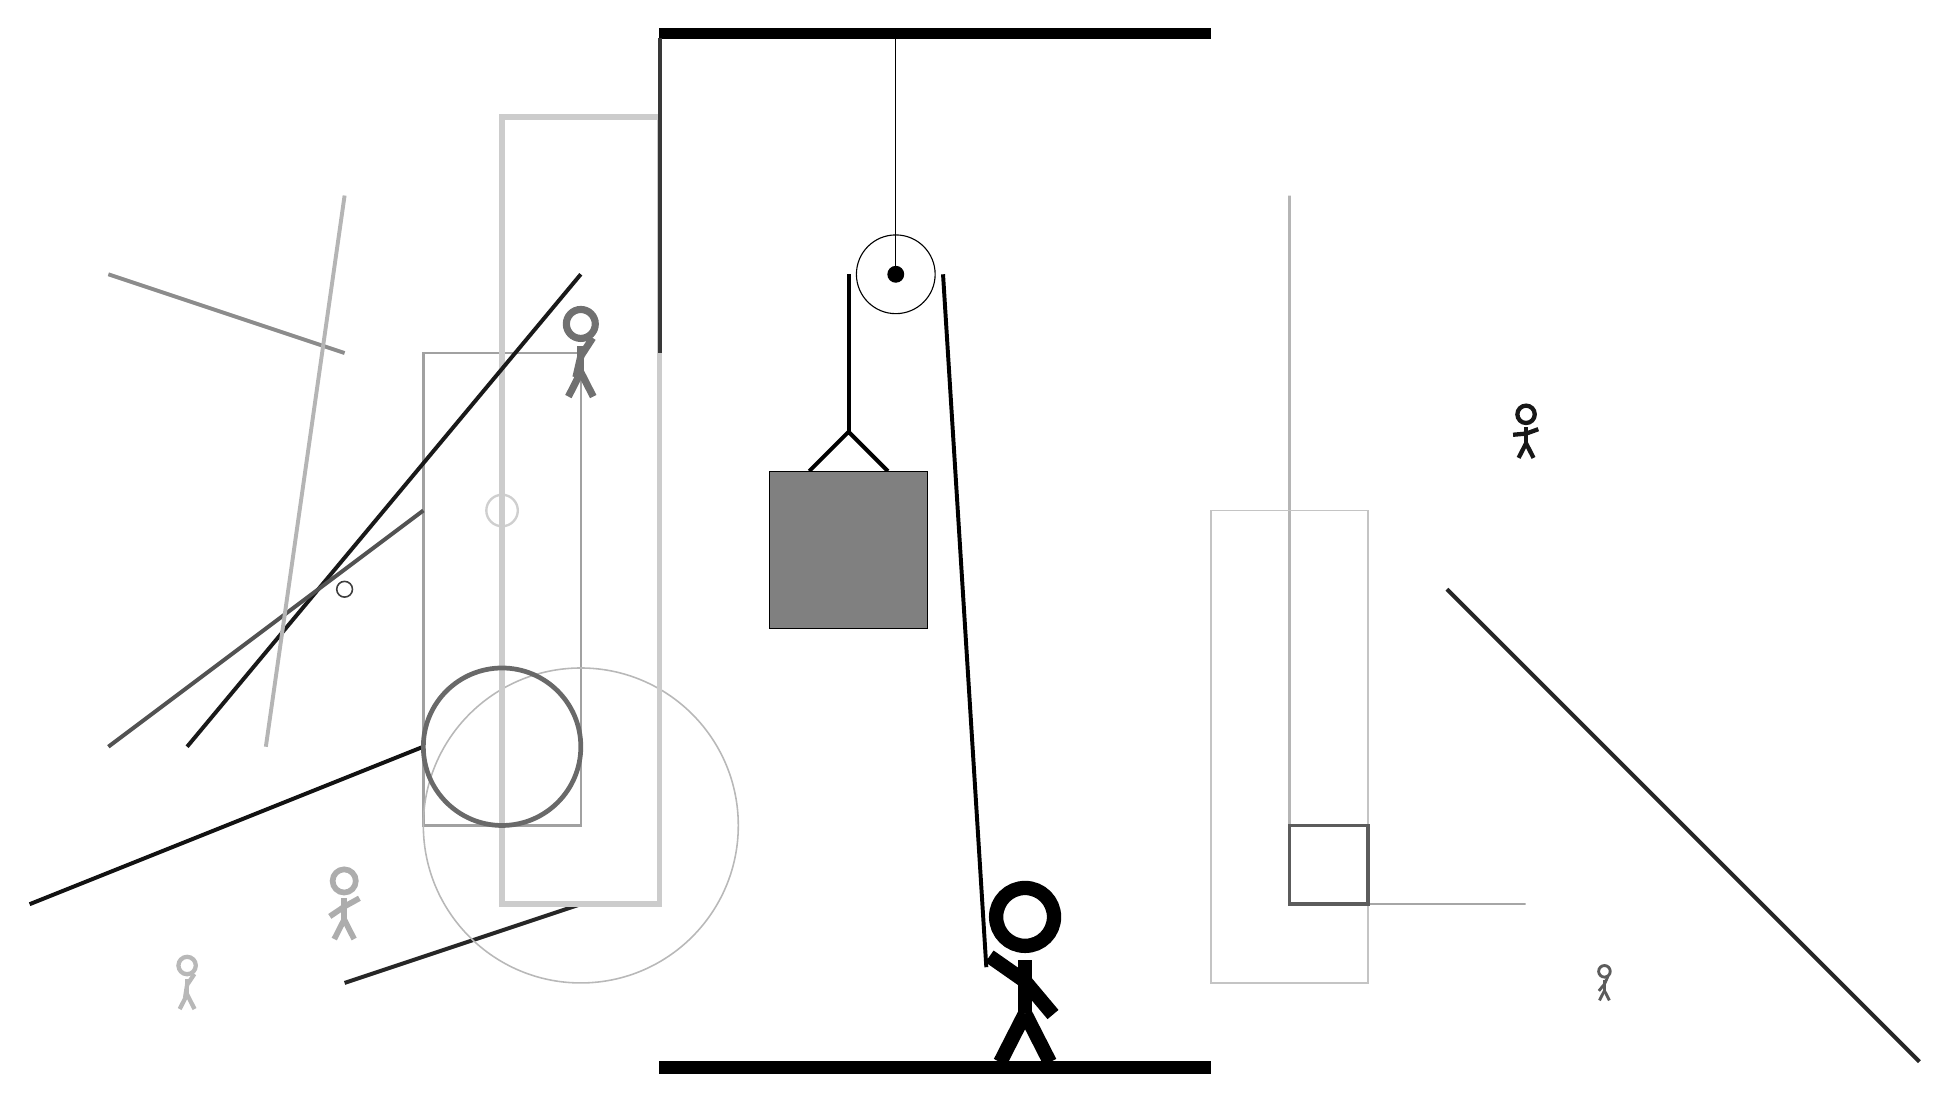
\begin{tikzpicture}
		%%%%% START %%%%%
		
		\draw[fill=black] (-2, 10) rectangle (5, 10.125);
		
		\draw (1, 7) circle (0.5);
		\draw[fill=black] (1, 7) circle (0.1);
		\draw (1, 10) -- (1, 7);
		
		\draw[line width=0.5mm] (-0.1, 4.5) -- (0.4, 5.0) -- (0.9, 4.5);
		\draw[fill=black!50] (-0.6, 4.5) rectangle (1.4, 2.5);
		
		\draw[line width=0.5mm] (0.4, 7) -- (0.4, 5.0);
		\centerarc[line width=0.5mm](1, 7)(0:180:0.6);
		\draw[line width=0.5mm](1.6, 7) -- (2.15, -1.8);
		
		\draw[line width=0.5mm, color=black!99] (5, -1) rectangle (5, -1);
		
		\draw[line width=0.5mm, color=black!85](-3, -1) -- (-6, -2);
		\draw[line width=0.3mm, color=black!37] (-3, 0) rectangle (-5, 6);
		\node[line width=0.5mm, color=black!64] at (10, -2) {\Strichmaxerl[2][50][66]};
		\draw [line width=0.3mm, color=black!19](-4, 4) circle (0.2);
		
		\node[line width=0.5mm, color=black!28] at (-8, -2) {\Strichmaxerl[3][81][56]};
		\draw[line width=0.5mm, color=black!93](-5, 1) -- (-10, -1);
		
		\draw [line width=0.2mm, color=black!28](-3, 0) circle (2.0);
		\draw[line width=0.5mm, color=black!85](8, 3) -- (14, -3);
		\draw[line width=0.7mm, color=black!20] (-4, -1) rectangle (-2, 9);
		\draw [line width=0.6mm, color=black!59](-4, 1) circle (1.0);
		\draw[line width=0.4mm, color=black!29] (6, 8) rectangle (6, 0);
		\node[line width=0.2mm, color=black!32] at (-6, -1) {\Strichmaxerl[4][34][29]};
		
		\draw[line width=0.3mm, color=black!35] (6, -1) rectangle (9, -1);
		\draw[line width=0.5mm, color=black!90](-3, 7) -- (-8, 1);
		\draw[line width=0.5mm, color=black!45](-6, 6) -- (-9, 7);
		
		\node[line width=0.7mm, color=black!56] at (-3, 6) {\Strichmaxerl[5][77][57]};
		
		\draw[line width=0.2mm, color=black!23] (5, 4) rectangle (7, -2);
		\draw[line width=0.5mm, color=black!78](-2, 10) -- (-2, 6);
		
		\draw[line width=0.5mm, color=black!68](-5, 4) -- (-9, 1);
		\draw[line width=0.5mm, color=black!64] (6, 0) rectangle (7, -1);
		\draw [line width=0.2mm, color=black!76](-6, 3) circle (0.1);
		\node[line width=0.2mm, color=black!91] at (9, 5) {\Strichmaxerl[3][5][20]};
		\draw[line width=0.5mm, color=black!29](-6, 8) -- (-7, 1);
		
		\node at (2.6, -1.9) {\Strichmaxerl[10][-35][-50]};
		
		\draw[fill=black] (-2, -3) rectangle (5, -3.15);
		
		%%%%% END %%%%%
	\end{tikzpicture}
\end{document}